\fullpageexercises[Exercise: Pythagorean Theorem via Dimensional Analysis]
{
\section*{Dimensional Analysis and Geometry}  
Contrary to my six-year-old child, who argues with his teachers that math is only about numbers and that geometry has nothing to do with it, the ancient Greeks developed geometry without numerical coordinates, relying on operations with geometric objects rather than arithmetic. Dimensional analysis follows this principle: physical laws can be viewed as relationships between both numbers and dimensioned quantities.
\section*{Objective}  
Derive $a^2 + b^2 = c^2$ using a dimensional argument involving area scaling.
\begin{enumerate}
    \item \textbf{Scaling Argument}  
    \newline
    A right triangle is uniquely determined by its hypotenuse $c$ and one acute angle $\phi$. The only dimensionally valid expression for its area is
    \[
    \Delta = c^2 f(\phi),
    \]
    where $f(\phi)$ is a dimensionless function.
    \textit{(Why $c$ rather than $a$ or $b$? By similarity, the shape depends on $\phi$ and a squared length. The hypotenuse $c$ is the natural candidate.)}
    \begin{center}
    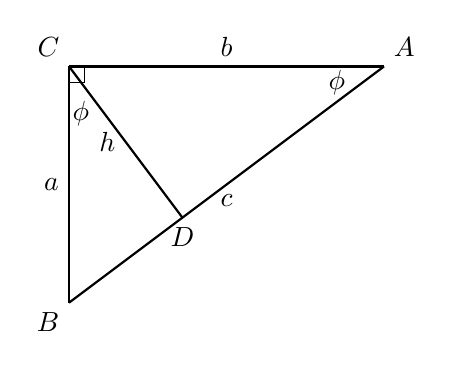
\begin{tikzpicture}[scale=1]
      % Define vertices for a 3-4-5 right triangle with right angle at C:
      \coordinate (B) at (0,0);
      \coordinate (C) at (0,3);
      \coordinate (A) at (4,3);
      
      % Compute foot D of the altitude from C to AB
      \coordinate (D) at (1.44,1.08);
      
      % Draw triangle ABC
      \draw[thick] (A) -- (B) node[midway, below] {$c$};
      \draw[thick] (B) -- (C) node[midway, left] {$a$};
      \draw[thick] (C) -- (A) node[midway, above] {$b$};
      
      % Label vertices
      \node[above right] at (A) {$A$};
      \node[below left] at (B) {$B$};
      \node[above left] at (C) {$C$};
      
      % Altitude from C to AB
      \draw[thick] (C) -- (D) node[midway, left] {$h$};
      \node[below] at (D) {$D$};
      
      % Right angle marker at C
      \draw (C) ++(0.2,0) -- ++(0,-0.2) -- ++(-0.2,0);
      
      % Acute angle at A
      \node at (3.4,2.8) {$\phi$};
      % Angle at C
      \node at (0.15,2.4) {$\phi$};
    
    \end{tikzpicture}
    \end{center}
    \item \textbf{Similar Triangles and Decomposition}  
    \newline
    The altitude $CD$ from $C$ to $AB$ divides the original right triangle $\triangle ABC$ into two smaller right triangles, $\triangle CBD$ and $\triangle ACD$. By angle-angle (AA) similarity:
    \[
    \triangle ABC \sim \triangle CBD \sim \triangle ACD.
    \]
    Because area scales as the square of a characteristic length, The sub-areas (corresponding to sides $a$ or $b$) take the form $\Delta_1 = a^2 f(\phi)$ and $\Delta_2 = b^2 f(\phi)$.
    Since the total area is additive,  
    \[
    c^2 f(\phi) = a^2 f(\phi) + b^2 f(\phi).
    \]
    
    \item \textbf{Conclusion}  
    Dividing by $f(\phi)$ (assumed nonzero) gives
    \[
    c^2 = a^2 + b^2.
    \]
\end{enumerate}
\section*{Mathematical Formalism of Dimensional Analysis}  
Dimensional analysis can be rigorously formalized using a graded algebraic structure where physical quantities lie in one-dimensional vector spaces $V^d$ indexed by a group $G$ of exponents (e.g., $\mathbb{R}^n$ for base units). Multiplication corresponds to the tensor product $V^a \otimes V^b \cong V^{a+b}$, and one only adds elements within the same space $V^d$. For example, a quantity in kilograms lies in $V^{(1,0,0,\ldots)}$ and one in meters per second lies in $V^{(1,0,-1,\ldots)}$, reflecting mass and velocity dimensions respectively. Physical laws hold under any consistent rescaling of units, leading to constraints like Buckingham's $\pi$-theorem.  
For details, see Tao (2012):  
\href{https://terrytao.wordpress.com/2012/12/29/a-mathematical-formalisation-of-dimensional-analysis/}{\textrm{https://bit.ly/tao\_dim}}
}